\documentclass{report}
\usepackage[colorlinks=true, linkcolor=blue]{hyperref}
\usepackage{graphicx}
\usepackage{subcaption}
\usepackage{amsmath}
\usepackage{float}
\usepackage[most]{tcolorbox}
\setcounter{tocdepth}{3}

\title{\Huge CS215 Assignment 2}
\author{Tamanna Kumari, 24B1015
\\\\Sagar V, 24B1021
\\\\Videep Reddy Jalapally, 24B1037}
\date{\today}

\begin{document}

\maketitle
\tableofcontents
\newpage

\section*{Question 4}
\addcontentsline{toc}{section}{Question 4}

\subsection*{Image 2 = 'T2.jpg'}
\addcontentsline{toc}{subsection}{Image 2 = 'T2.jpg'}

\subsubsection*{Correlation Coefficient \boldmath$\rho$}
\addcontentsline{toc}{subsubsection}{Correlation Coefficient $\rho$}

\begin{figure}[h]
    \centering
    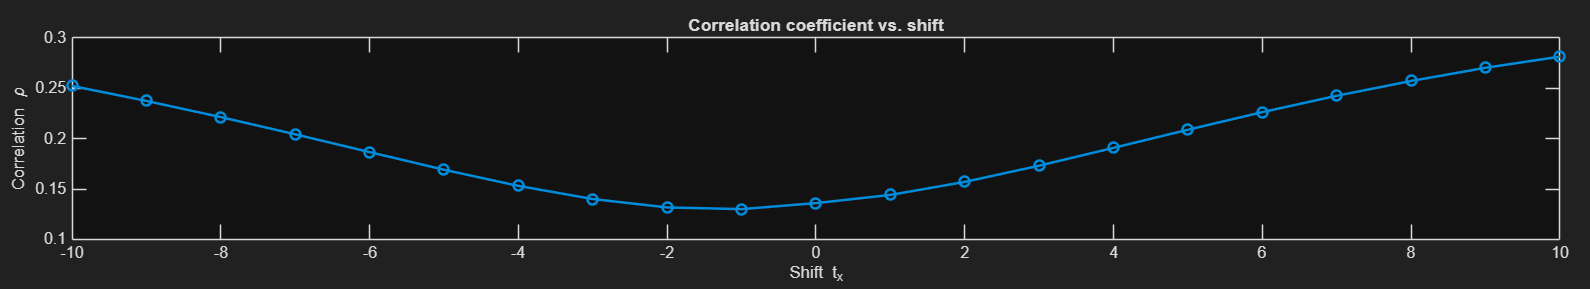
\includegraphics[width=\textwidth]{q4_0_corr.png}
    \caption{Graph between $\rho$ and $t_x$}
\end{figure}

The two images, \texttt{T1.jpg} and \texttt{T2.jpg}, are contrast MRI scans of the brain. In one image, gray matter appears dark while white matter is bright, and in the other this contrast is reversed. As a result, the relationship between corresponding pixels is inherently non-linear. When the shift is increased in either direction, this non-linear correspondence begins to blur, since we start comparing non-corresponding pixels. This leads to a higher average correspondence overall, which partly counteracts the strong lack of dependence observed between the truly corresponding pixels.

\vspace{1em}

\subsubsection*{Quadratic Mutual Information \textit{QMI}}
\addcontentsline{toc}{subsubsection}{Quadratic Mutual Information \textit{QMI}}

\begin{figure}[h]
    \centering
    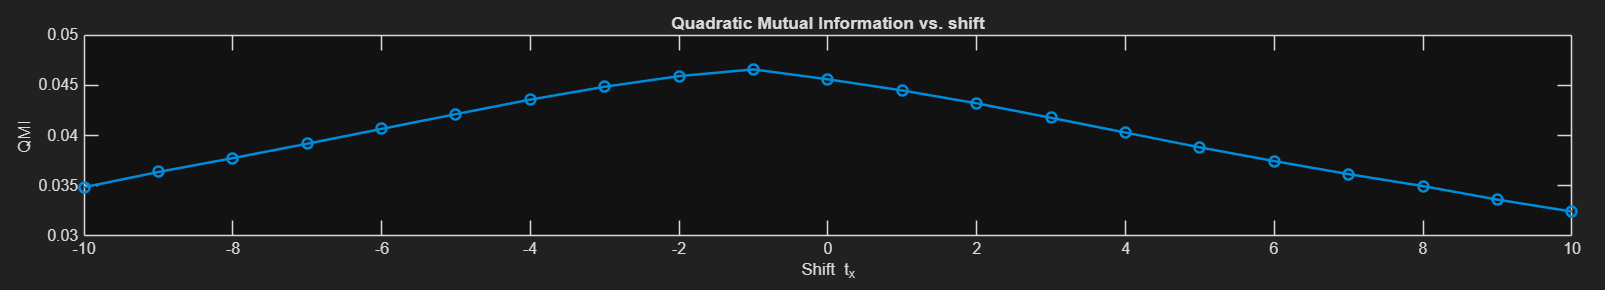
\includegraphics[width=\textwidth]{q4_0_qmi.png}
    \caption{Graph between \textit{QMI} and $t_x$}
\end{figure}

QMI reaches its peak at around $t_x = 0$, indicating strong statistical dependence between corresponding pixels. Although this relationship is non-linear, as seen in the $\rho$ vs. $t_x$ graph, it remains consistent across the image. This explains why QMI is maximized when the images are aligned. As $t_x$ shifts further in either direction, the correspondence fades, since non-corresponding pixels are being compared and no clear relationship exists. However, the decline is gradual rather than abrupt, because neighboring pixels still share some degree of similarity.

\vspace{1em}

\newpage
\subsubsection*{Mutual Information \textit{MI}}
\addcontentsline{toc}{subsubsection}{Mutual Information \textit{MI}}

\begin{figure}[h]
    \centering
    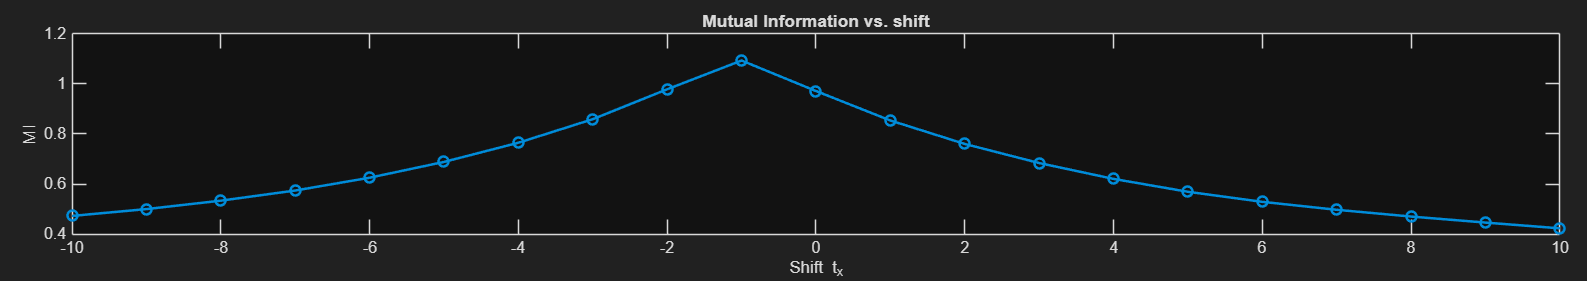
\includegraphics[width=\textwidth]{q4_0_mi.png}
    \caption{Graph between \textit{MI} and $t_x$}
\end{figure}

Mutual Information is another measure of statistical dependence between two quantities. Similar to \textit{QMI}, it reaches its peak near $t_x = 0$, where the corresponding pixels of the two images maintain a consistent relationship, as they are contrast MRIs of the same region. However, as $|t_x|$ increases, MI drops much more sharply. Since it is based on a logarithmic summation, the measure is highly sensitive and shows a strong peak under strong dependence but declining rapidly with even slight deviations. In contrast, \textit{QMI} tends to smooth out these variations, while MI produces sharper peaks due to the nature of its summation.

\vspace{2em}

\subsection*{\boldmath$I_2 = 255 - I_1$}
\addcontentsline{toc}{subsection}{I_2 = 255 - I_1}

Here, the second image that we are using is a perfect negative of the first as we directly write $I2 = 255 - I1$.

\subsubsection*{Correlation Coefficient \boldmath$\rho$}
\addcontentsline{toc}{subsubsection}{Correlation Coefficient $\rho$}

\begin{figure}[h]
    \centering
    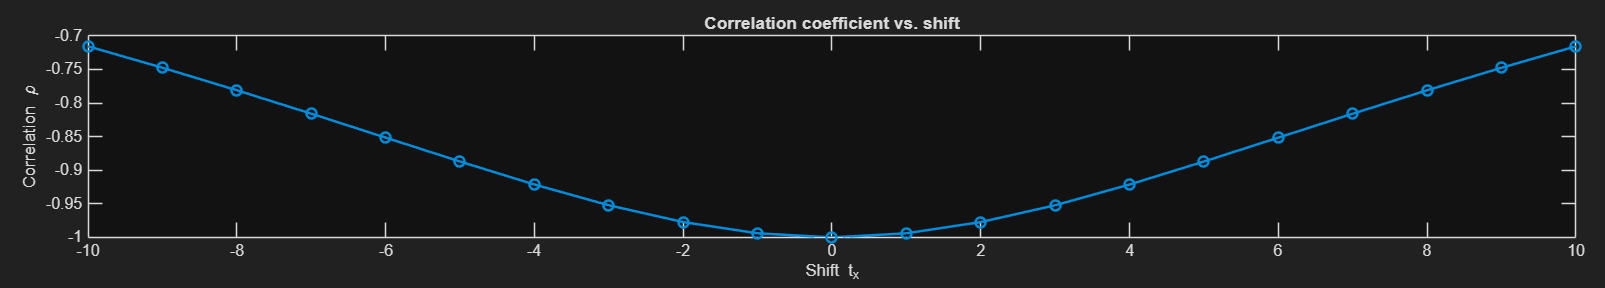
\includegraphics[width=\textwidth]{q4_1_corr.png}
    \caption{Graph between $\rho$ and $t_x$}
\end{figure}

At $t_x = 0$, the correlation is exactly $-1$, since we explicitly defined the relation as $I_2 = 255 - I_1$, which represents a perfect negative linear relation. The intensities of corresponding pixels therefore follow an exact linear dependence. As $|t_x|$ increases, however, this correspondence begins to blur, as we are no longer comparing strictly aligned pixels but rather neighbouring ones. Consequently, the value of $\rho$ decreases, though not sharply, since neighbouring pixels often share similar intensity values with their corresponding counterparts.

\vspace{1em}

\subsubsection*{Quadratic Mutual Information \textit{QMI}}
\addcontentsline{toc}{subsubsection}{Quadratic Mutual Information \textit{QMI}}

\begin{figure}[h]
    \centering
    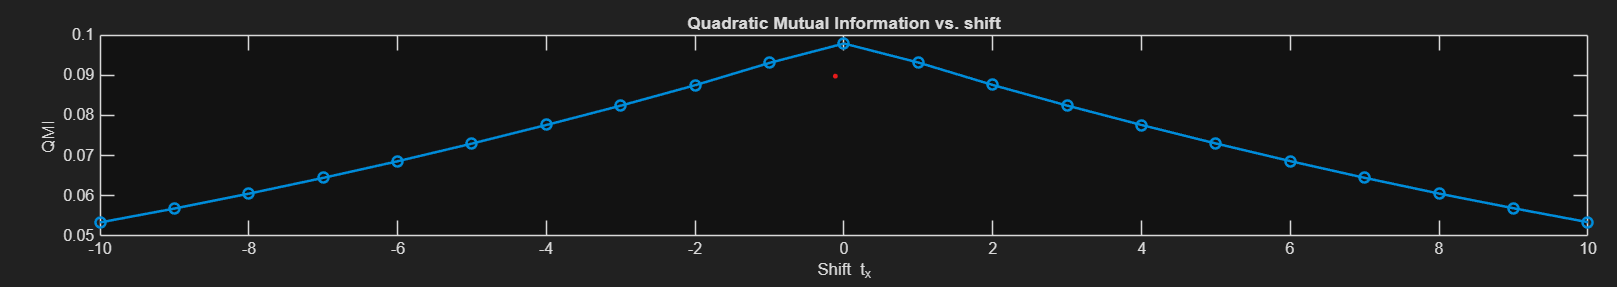
\includegraphics[width=\textwidth]{q4_1_qmi.png}
    \caption{Graph between \textit{QMI} and $t_x$}
\end{figure}

\textit{QMI} is the highest at $t_x = 0$, showing the consistent negative linear relation between corresponding pixels in the two images. As $|t_x|$ increases, the relationship tends to fall off as the neighbouring pixels are not as closely related as the corresponding ones. But still there is somewhat of a relation between them as the neighbouring pixels tend to have similar intensities. As expected, \textit{QMI} falls to its lowest value at $|t_x| = 10$.

\vspace{1em}

\subsubsection*{Mutual Information \textit{MI}}
\addcontentsline{toc}{subsubsection}{Mutual Information \textit{MI}}

\begin{figure}[h]
    \centering
    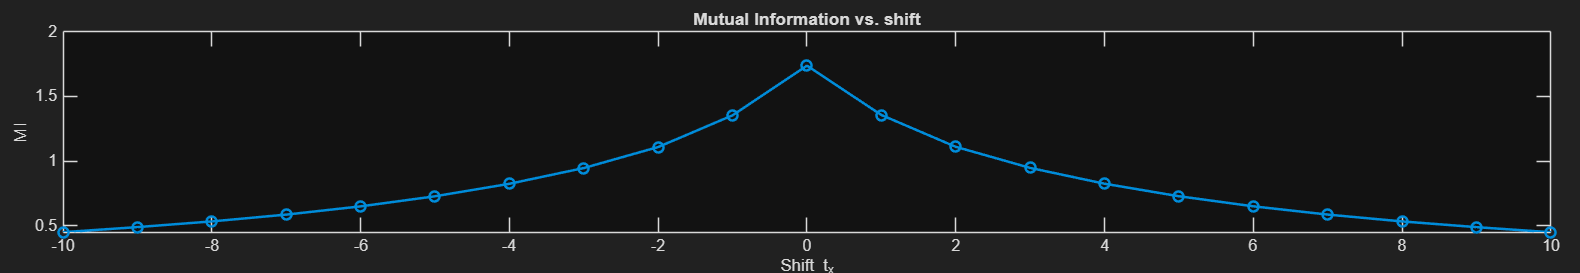
\includegraphics[width=\textwidth]{q4_1_mi.png}
    \caption{Graph between \textit{MI} and $t_x$}
\end{figure}

\textit{MI} has a similar graph to \textit{QMI} but here the value drop is much steeper as compared to \textit{QMI}. This is due to the logarithmic summation used in \textit{MI}, which produces very high peaks when there is a strong dependence, yet these peaks drop off rapidly as the relationship becomes even slightly inconsistent. As expected, the values reach their minimum at $|t_x| = 10$.

\newpage

\subsection*{\boldmath$I_2 = 255 * (I_1)^2 / \max((I_1)^2) + 1$}
\addcontentsline{toc}{subsection}{$I_2 = 255 * (I_1)^2 / \max((I_1)^2) + 1$}

Here, the intensity of the corresponding pixel in the second image is scaled as the normalized square of the intensity of the pixel in the first image. This increases the observed difference due to intensity values while keeping the min and max the same.

\subsubsection*{Correlation Coefficient \boldmath$\rho$}
\addcontentsline{toc}{subsubsection}{Correlation Coefficient $\rho$}

\begin{figure}[h]
    \centering
    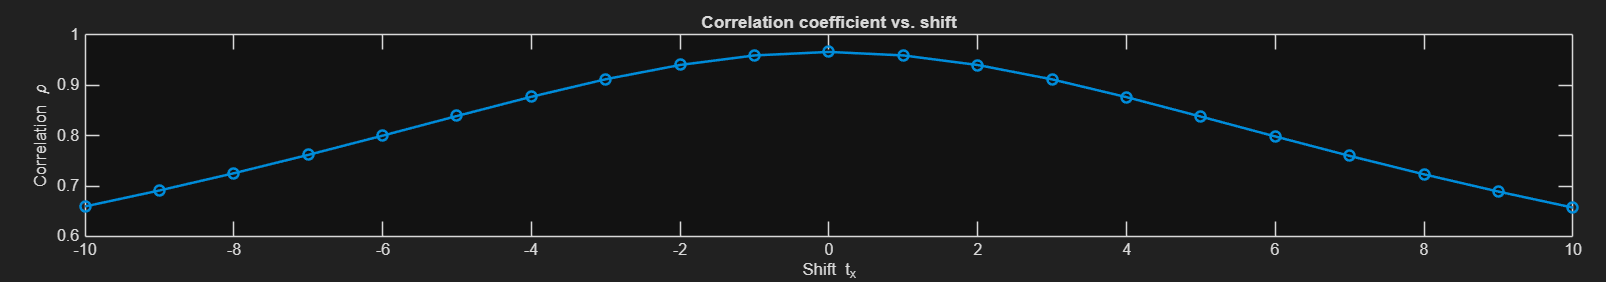
\includegraphics[width=\textwidth]{q4_2_corr.png}
    \caption{Graph between $\rho$ and $t_x$}
\end{figure}

The squaring operation reduces the difference in the low-mid intensity value pixels whereas it blows up the difference between the high and mid intensity value pixels. This makes the transformed image look more biased towards its brighter regions while still maintaining a linear correspondence. Hence, it peaks at $t_x = 0$. Similarly, $\rho$ drops as $|t_x|$ increases and reaches it's lowest value at $|t_x| = 10$ as expected.

\vspace{1em}

\subsubsection*{Quadratic Mutual Information \textit{QMI}}
\addcontentsline{toc}{subsubsection}{Quadratic Mutual Information \textit{QMI}}

\begin{figure}[h]
    \centering
    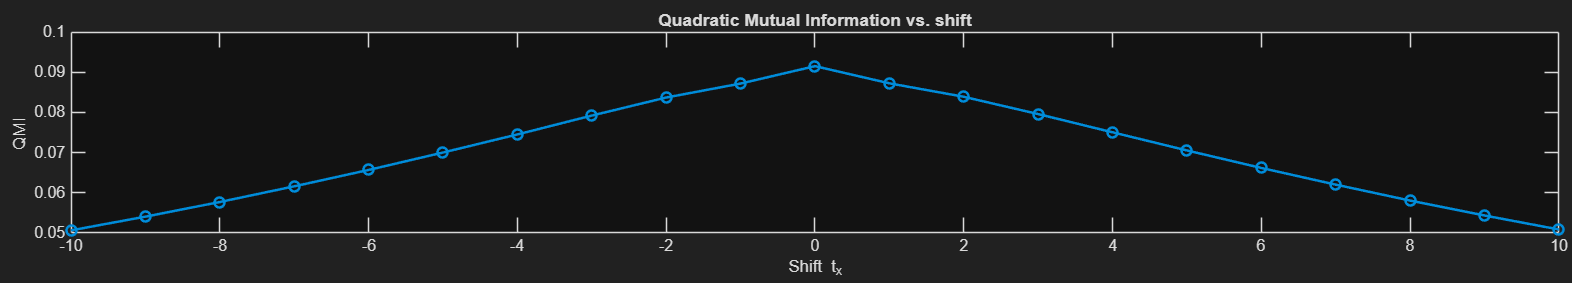
\includegraphics[width=\textwidth]{q4_2_qmi.png}
    \caption{Graph between \textit{QMI} and $t_x$}
\end{figure}

Similar to the above cases, \textit{QMI} peaks at $t_x = 0$ as there is a consistent relation between corresponding pixels. But as $|tx|$ increases, this relationship becomes less and less defined as we now start comaparing the neighbouring pixels instead of the corresponding pixels in the two images. Hence, as expected, it symmetrically reaches a lowest value at $|t_x| = 10$.

\newpage

\subsubsection*{Mutual Information \textit{MI}}
\addcontentsline{toc}{subsubsection}{Mutual Information \textit{MI}}

\begin{figure}[h]
    \centering
    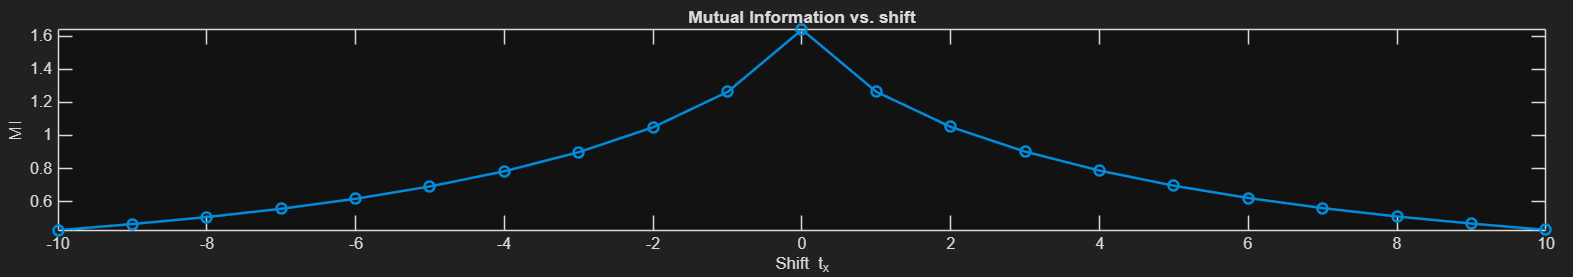
\includegraphics[width=\textwidth]{q4_2_mi.png}
    \caption{Graph between \textit{MI} and $t_x$}
\end{figure}

\textit{MI} plot is similar to \textit{QMI} plot but here the peak at $t_x = 0$ is much higher compared to it's surrounding values. As we saw earlier, \textit{MI} tends to have very strong peaks at strong dependence but these peaks diminish quickly as relation becomes even a little inconsistent. In these images, since we are using the square relation to compute intensity values of second image, the fall off in dependence is much higher as compared to earlier cases. This causes there to be a visible high peak higher than any other plot we've obtained so far. As expected, it reaches its lowest value at $|t_x| = 10$.

\end{document}
